\documentclass[conference]{IEEEtran}
\IEEEoverridecommandlockouts

\usepackage{iftex}
\ifXeTeX
  % Tectonic builds with XeTeX; use a Times clone so the output matches the
  % pdfLaTeX (Overleaf) build of IEEEtran.
  \usepackage{fontspec}
  \setmainfont{texgyretermes}[Extension=.otf, UprightFont=*-regular,
    BoldFont=*-bold, ItalicFont=*-italic, BoldItalicFont=*-bolditalic]
  \setsansfont{texgyreheros}[Extension=.otf, UprightFont=*-regular,
    BoldFont=*-bold, ItalicFont=*-italic, BoldItalicFont=*-bolditalic]
  \setmonofont{texgyrecursor}[Extension=.otf, UprightFont=*-regular,
    BoldFont=*-bold, ItalicFont=*-italic, BoldItalicFont=*-bolditalic]
\fi
\usepackage{cite}
\usepackage{amsmath,amssymb,amsfonts}
\usepackage{graphicx}
\usepackage{booktabs}
\usepackage{array}
\usepackage{xcolor}
\usepackage{url}
\usepackage{tikz}
\usetikzlibrary{arrows.meta,positioning,fit,calc}

% Placeholder number macros. experiments/make_paper_assets.py (Task 18) overwrites
% this file with values computed from results/. Never type a result by hand.
\newcommand{\TBD}{\textbf{[TBD]}}
% --- fixed-alpha baseline (chosen on pooled dev, per encoder)
\newcommand{\AlphaStarBge}{\TBD}
\newcommand{\AlphaStarGemma}{\TBD}
% --- QAF training
\newcommand{\QAFnDev}{\TBD}          % pooled dev queries used to fit QAF
\newcommand{\QAFtrainRsq}{\TBD}      % training R^2 of the ridge model
\newcommand{\QAFtopFeature}{\TBD}    % feature with the largest |coefficient|
\newcommand{\QAFlatencyMs}{\TBD}     % mean added latency of QAF (features + predict), ms
% --- headline retrieval gains (nDCG@10, qaf+rr minus hybrid_fixed+rr)
\newcommand{\QAFgainSciFact}{\TBD}
\newcommand{\QAFgainFiQA}{\TBD}
\newcommand{\QAFgainHotpot}{\TBD}
\newcommand{\QAFgainRFC}{\TBD}
\newcommand{\QAFpRFC}{\TBD}          % one-sided paired bootstrap p, RFC
\newcommand{\QAFpSciFact}{\TBD}
% --- hybrid vs single retrievers (nDCG@10)
\newcommand{\HybridGainOverDenseRFC}{\TBD}
\newcommand{\HybridGainOverBMRFC}{\TBD}
\newcommand{\BestNDCGRFC}{\TBD}
\newcommand{\BestNDCGSciFact}{\TBD}
\newcommand{\BMndcgSciFact}{\TBD}    % sanity check against published BEIR BM25
% --- oracle headroom (oracle alpha minus fixed alpha*, nDCG@10)
\newcommand{\OracleHeadroomSciFact}{\TBD}
\newcommand{\OracleHeadroomRFC}{\TBD}
% --- reranking and latency
\newcommand{\RerankGainSciFact}{\TBD}
\newcommand{\RerankLatencyMs}{\TBD}
\newcommand{\TotalLatencyMs}{\TBD}
% --- Matryoshka (EmbeddingGemma 2)
\newcommand{\MatryoshkaDropTwoFiftySix}{\TBD} % nDCG@10 drop from 768 to 256 dims
\newcommand{\MatryoshkaIndexMBOneTwentyEight}{\TBD}
% --- generation
\newcommand{\GenN}{\TBD}             % questions per dataset in generation eval
\newcommand{\RagasN}{\TBD}           % RAGAS sample size
\newcommand{\GenFoneQAF}{\TBD}
\newcommand{\GenFoneDense}{\TBD}
\newcommand{\GenEMQAF}{\TBD}
\newcommand{\FaithQAF}{\TBD}
\newcommand{\FaithDense}{\TBD}


% Results tables/figures are produced by experiments/make_paper_assets.py.
% Until they exist the paper still builds, with a visible placeholder.
\newcommand{\inputtable}[1]{%
  \IfFileExists{tables/#1.tex}{\input{tables/#1}}{%
    \begin{table}[t]\centering\caption{[\detokenize{#1} table pending]}\label{tab:#1}\fbox{\parbox{0.9\columnwidth}{\centering\small Table \texttt{tables/\detokenize{#1}.tex} not generated yet.}}\end{table}}}
\newcommand{\inputfigure}[2]{%
  \IfFileExists{figures/#1.pdf}{%
    \begin{figure}[t]\centering\includegraphics[width=0.62\columnwidth]{figures/#1}\caption{#2}\label{fig:#1}\end{figure}}{%
    \begin{figure}[t]\centering\fbox{\parbox{0.9\columnwidth}{\centering\small Figure \texttt{figures/\detokenize{#1}.pdf} not generated yet.}}\caption{#2}\label{fig:#1}\end{figure}}}

\begin{document}

\title{Query-Adaptive Hybrid Retrieval for Retrieval-Augmented Generation on Identifier-Heavy Corpora}

\author{
\IEEEauthorblockN{Parth Tuteja}
\IEEEauthorblockA{\textit{Dept. of Computer Science}\\ \textit{and Engineering}\\
\textit{Chitkara University}\\
Punjab, India\\
2310991172}
\and
\IEEEauthorblockN{Reetika}
\IEEEauthorblockA{\textit{Dept. of Computer Science}\\ \textit{and Engineering}\\
\textit{Chitkara University}\\
Punjab, India\\
2310991267}
\and
\IEEEauthorblockN{Rishabh Puri}
\IEEEauthorblockA{\textit{Dept. of Computer Science}\\ \textit{and Engineering}\\
\textit{Chitkara University}\\
Punjab, India\\
2310991269}
}

\maketitle

\begin{abstract}
% TODO: write after results are in (about 200 words). Must stay consistent with
% the approved project abstract ("Team 39 - Abstract Hybrid Retrieval RAG.pdf"):
% problem (static LLM knowledge, hallucination) -> RAG bounded by retrieval ->
% dense vs sparse failure modes -> hybrid pipeline (structural chunking, BM25 +
% HNSW dense index, weighted RRF, cross-encoder rerank, local 7B generator).
% Add what is new relative to the approved abstract: QAF (LLM-free per-query
% fusion weight) and EmbeddingGemma 2 (with Matryoshka sizes). Quote the
% headline numbers only through numbers.tex macros, e.g. \QAFgainRFC,
% \HybridGainOverDenseRFC, \QAFlatencyMs, \GenFoneQAF.
\textbf{[Abstract pending results.]}
\end{abstract}

\begin{IEEEkeywords}
retrieval-augmented generation, hybrid retrieval, reciprocal rank fusion,
query-adaptive fusion, BM25, dense retrieval, cross-encoder reranking
\end{IEEEkeywords}

\section{Introduction}
\label{sec:intro}

Large language models answer fluently, but what they know is fixed at training
time. They have not seen documents written after their cutoff or anything
kept inside an organisation, and when a question falls outside what they
learned they tend to produce a confident wrong
answer~\cite{ji2023hallucination}. Retrieval-augmented generation
(RAG)~\cite{lewis2020rag,gao2023ragsurvey} fetches relevant passages at query
time and asks the model to answer from them, which moves the burden onto the
retriever: if the passage that holds the answer is not retrieved, the
generator cannot recover it.

The two common retriever families fail in different places. Dense
retrievers~\cite{karpukhin2020dpr} match meaning and handle paraphrase well,
but they often miss exact strings that were rare in their training data,
such as version numbers or header names. A question about a status code can
be answered from one line of one specification, and to an embedding model
that line may look much like dozens of other passages on the same topic. BM25~\cite{robertson2009bm25} finds such
strings easily, but it fails when the question and the source use different
words. Hybrid retrieval runs both and merges the results, usually with
Reciprocal Rank Fusion (RRF)~\cite{cormack2009rrf}, with one constant
balance between the two sides. That constant is a compromise between queries
that need exact matching and queries that need semantic matching.

Choosing the balance per query is not a new idea. DAT~\cite{hsu2025dat} asks
an LLM to judge the top result of each retriever and sets the weight from
those judgements. That works, but it puts LLM calls on the retrieval path of
every query. We ask whether cheap signals from the query text and the two
candidate lists are enough. Our
method, Query-Adaptive Fusion (QAF), feeds 12 such features to a ridge
regression that outputs the fusion weight. It is trained once on development
queries, needs no LLM at query time, and its coefficients can be read off
directly. In our experiments the answer is mostly no. QAF is cheap and
readable, but it does not reliably beat a well-chosen fixed weight, and we
report this result together with an analysis of why.

We build a complete pipeline, from structural
chunking through BM25 and dense indexing, weighted RRF and cross-encoder
reranking to a local 7B generator. Everything runs on a single laptop. We test
it on three public collections and on a new corpus of 20 IETF RFCs, with two
encoders: BGE-small and Google's recent EmbeddingGemma~2. Our contributions
are:
\begin{itemize}
  \item \textbf{QAF}, an LLM-free, interpretable predictor of the per-query
  dense/sparse fusion weight, trained on a plateau-centre regression
  target derived from per-query weight sweeps, together with an analysis of
  why it does not reliably beat a tuned fixed weight even though per-query
  headroom exists.
  \item \textbf{An identifier-heavy RFC test collection} of 2{,}973 chunks and
  101 questions, generated with a local LLM, filtered automatically and
  checked by all three authors, with relevance labels derived from answer
  spans.
  % NOTE(results, part 2): add "an ablation" / "EmbeddingGemma 2 at four
  % embedding sizes" back to this bullet only if Task 14 produces them.
  \item \textbf{A controlled comparison} of sparse, dense, fixed-weight hybrid
  and QAF retrieval, with and without reranking, on four collections and two
  encoders, with paired bootstrap tests. It shows that fusion helps when the
  two retrievers are comparably strong, that BM25 is the strongest single
  retriever on identifier-heavy RFC text, and that reranking can hurt a
  strong first stage.
  % NOTE(results, part 2): keep "answer quality ... judged faithfulness" only if
  % Task 15 (generation, RAGAS) produces results.
  \item \textbf{An end-to-end account of cost}: per-stage latency and answer
  quality (exact match, F1 and judged faithfulness) on commodity hardware
  with no paid API.
\end{itemize}

Section~\ref{sec:related} reviews related work. Section~\ref{sec:method}
describes the pipeline and QAF, and Section~\ref{sec:setup} the data,
configurations and metrics. Section~\ref{sec:results} reports results,
Section~\ref{sec:discussion} discusses them along with the limitations of the
study, and Section~\ref{sec:conclusion} concludes.

\section{Related Work}
\label{sec:related}

\subsection{Sparse and dense retrieval}
BM25~\cite{robertson2009bm25} remains a strong baseline; on the BEIR
zero-shot benchmark~\cite{thakur2021beir} it beats many neural retrievers
outside their training domain. Its weakness is vocabulary mismatch, which dense
retrievers address by encoding queries and passages into one vector space. DPR~\cite{karpukhin2020dpr} trained a BERT bi-encoder on
question--passage pairs and clearly outperformed BM25 on open-domain QA, and
Sentence-BERT~\cite{reimers2019sbert} made such bi-encoders easy to train and
use. ColBERT~\cite{khattab2020colbert} keeps one vector per token and scores
by late interaction, which recovers some exact-match behaviour at the price of
a much larger index. Among general-purpose embedders, the BGE models from the
C-Pack release~\cite{xiao2024cpack} are small and strong on English retrieval,
and EmbeddingGemma~\cite{vera2025embeddinggemma}
and its multimodal successor EmbeddingGemma~2~\cite{vera2026embeddinggemma2}
target on-device use. Both Gemma models are trained with Matryoshka
representation learning~\cite{kusupati2022matryoshka}, so the embedding can be
truncated to trade accuracy for memory. We use one encoder from each family and measure that
trade-off on our own collections.

\subsection{Hybrid retrieval and fusion}
Because the two families fail on different queries, combining them is an old
idea. Reciprocal Rank Fusion~\cite{cormack2009rrf} merges ranked lists using
only ranks and needs no score calibration, which is why it is the default in
most toolkits. Kuzi et al.~\cite{kuzi2020hybrid} showed that lexical and semantic
matching find different relevant documents, so running both raises recall, and Pyserini~\cite{lin2021pyserini} made sparse, dense and hybrid runs
reproducible with one toolkit. Bruch et al.~\cite{bruch2023fusion} compared
fusion functions in detail and found that a tuned convex combination of
normalised scores can beat RRF, and that RRF is sensitive to its parameters.
All of these use one setting for every query.

Per-query weighting is the closest prior work to ours. DAT~\cite{hsu2025dat}
asks an LLM to rate the top-1 result of the dense and the sparse retriever for
each query and turns the two ratings into the fusion weight. It reports gains
over fixed weighting, but every query costs extra LLM calls, which adds
latency and makes the system depend on a generator being available at
retrieval time. QAF targets the same decision with a different budget: a
linear model over cheap query and score statistics, trained once on dev
labels, with no model call at query time and coefficients that can be read
directly.

\subsection{Reranking and retrieval-augmented generation}
Cross-encoders read the query and passage together and are much more accurate
than bi-encoders, but too slow to run over a whole corpus;
Nogueira and Cho~\cite{nogueira2019passage} established the now standard
pattern of reranking a short candidate list with BERT. On the generation side,
DrQA~\cite{chen2017drqa} paired a TF-IDF retriever with a neural reader, and
RAG~\cite{lewis2020rag} trained a dense retriever and a generator together.
Gao et al.~\cite{gao2023ragsurvey} survey the pipeline variants that
followed, and Ji et al.~\cite{ji2023hallucination} review the unsupported
content that grounding is meant to reduce. Ma et al.~\cite{ma2023rewriting} rewrite the query before
retrieval; our optional expansion step is a simpler, untrained form of the
same idea. For evaluation without reference answers, RAGAS~\cite{es2024ragas}
uses an LLM judge to score faithfulness and relevance.

\subsection{Vectorless retrieval}
PageIndex~\cite{vectify2025pageindex} skips both indexes: an LLM builds a
table-of-contents tree for each long document and then reasons down the tree to
find the relevant section. This suits long, well-structured documents such as
RFCs, but every query costs several LLM calls. We cite it as the reasoning-based
extreme of the design space; our pipeline sits at the other end, where each
query costs two index look-ups, a linear model and one reranker pass.

\section{Method}
\label{sec:method}

Fig.~\ref{fig:pipeline} shows the pipeline. Each passage is indexed twice, in
BM25 and in a dense vector index. A query goes to both retrievers, their top-100
lists are merged by weighted Reciprocal Rank Fusion (RRF) with a weight that is
either constant or, in our method, predicted per query, and a cross-encoder
reorders the head of the fused list before the top five passages reach the
generator.

\begin{figure*}[t]
\centering
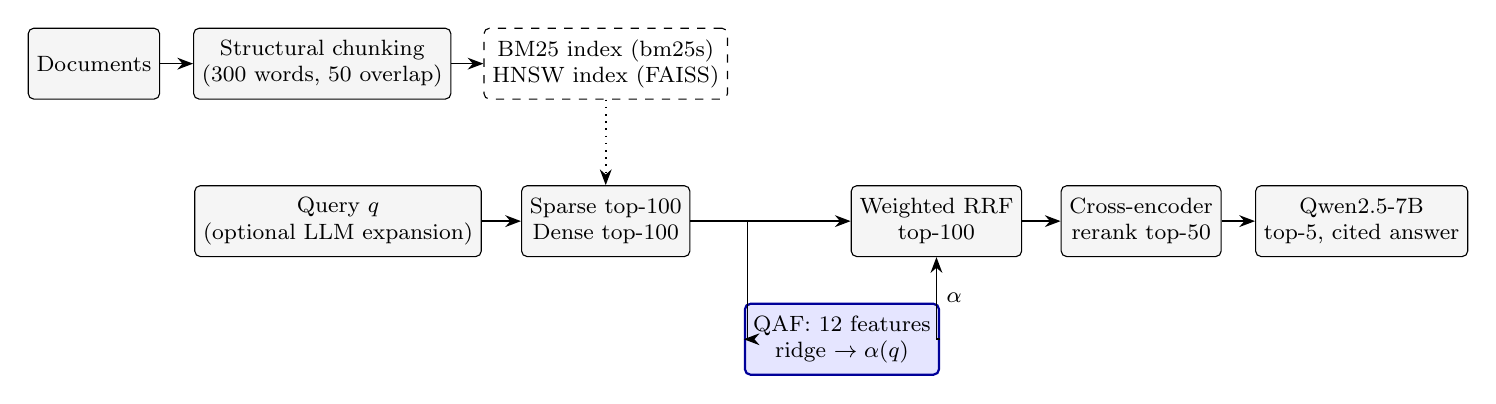
\begin{tikzpicture}[
  font=\footnotesize,
  box/.style={draw, rounded corners=2pt, align=center, minimum height=9mm, inner sep=3pt, fill=gray!8},
  ours/.style={box, fill=blue!10, draw=blue!60!black, thick},
  store/.style={box, fill=white, dashed},
  arr/.style={-{Stealth[length=2mm]}, semithick}]
  % offline row
  \node[box]   (docs)  at (-3.1,2.0) {Documents};
  \node[box]   (chunk) at (-0.2,2.0) {Structural chunking\\(300 words, 50 overlap)};
  \node[store] (idx)   at (3.4,2.0)  {BM25 index (bm25s)\\HNSW index (FAISS)};
  \draw[arr] (docs) -- (chunk);
  \draw[arr] (chunk) -- (idx);
  % query row
  \node[box]  (q)    at (0,0)    {Query $q$\\(optional LLM expansion)};
  \node[box]  (lists) at (3.4,0) {Sparse top-100\\Dense top-100};
  \coordinate (join) at (5.2,0);
  \node[ours] (qaf)  at (6.4,-1.5) {QAF: 12 features\\ridge $\rightarrow \alpha(q)$};
  \node[box]  (rrf)  at (7.6,0)  {Weighted RRF\\top-100};
  \node[box]  (rr)   at (10.2,0) {Cross-encoder\\rerank top-50};
  \node[box]  (gen)  at (13.0,0) {Qwen2.5-7B\\top-5, cited answer};
  \draw[arr] (q) -- (lists);
  \draw[arr, dotted] (idx) -- (lists);
  \draw[semithick] (lists.east) -- (join);
  \draw[arr] (join) -- (rrf.west);
  \draw[arr] (join) |- (qaf.west);
  \draw[arr] (qaf.east) -| node[pos=0.75, right]{$\alpha$} (rrf.south);
  \draw[arr] (rrf) -- (rr);
  \draw[arr] (rr) -- (gen);
\end{tikzpicture}
\caption{Pipeline. Top: offline indexing. Bottom: query time. The shaded block
is Query-Adaptive Fusion (QAF), which sets the dense weight $\alpha$ of the
fusion step separately for every query.}
\label{fig:pipeline}
\end{figure*}

\subsection{Chunking}
\label{sec:chunking}
BEIR and HotpotQA passages are already short and are indexed as they are.
Chunking matters for the RFC corpus, where one document can run past 100
pages. Our chunker splits the cleaned text into blocks at blank lines. A
one-line block is a heading if it is a numbered title of at most 12 words that
does not end in a period, colon or comma (``4.2.1 Frame Header''), or a short
line of at most 8 words that starts with a capital and contains only letters
and spaces. A heading closes the current chunk and becomes the first line of
the next, so section names are indexed with their bodies. Paragraphs are added
until the chunk would pass 300 words (hard ceiling 380); longer paragraphs are
split at sentences, then into word windows. Consecutive chunks of the same
section share 50 words of overlap. Each chunk is a verbatim slice of its source
and stores its character offsets, which we use for relevance labels. An
optional break on low embedding similarity between paragraphs was off in every
reported run, so boundaries follow document structure only.

\subsection{Sparse retrieval}
BM25 scores the title and text of each passage with the Lucene variant
implemented in \texttt{bm25s}~\cite{lu2024bm25s}:
\begin{equation}
  s_{\mathrm{BM25}}(q,d)=\sum_{t\in q}\mathrm{idf}(t)\,
  \frac{f(t,d)}{f(t,d)+k_1\!\left(1-b+b\,\frac{|d|}{\mathrm{avgdl}}\right)},
  \label{eq:bm25}
\end{equation}
where $f(t,d)$ is the frequency of $t$ in $d$ and
$\mathrm{idf}(t)=\ln\bigl(1+\frac{N-n_t+0.5}{n_t+0.5}\bigr)$ for $N$ passages,
$n_t$ of which contain $t$~\cite{robertson2009bm25}; $k_1=1.2$, $b=0.75$.

The tokenizer is where we departed most from defaults. The default
\texttt{bm25s} tokenizer keeps only runs of two or more word characters, so
\texttt{HTTP/2} becomes \texttt{http} and the version number, often exactly
what an RFC question asks about, is lost. Ours lowercases the text and
first matches compounds, alphanumeric runs joined by \texttt{.}, \texttt{\_},
\texttt{/}, \texttt{:} or \texttt{-}, and emits each compound both whole and as
its parts (\texttt{http/2} gives \texttt{http/2}, \texttt{http}, \texttt{2}).
Purely alphabetic tokens go through an English stopword list and the Snowball
stemmer; tokens with a digit or separator are never stemmed or dropped. The
same function serves documents, queries and the IDF look-ups used by QAF.

\subsection{Dense retrieval}
We compare two bi-encoders: BGE-small-en-v1.5~\cite{xiao2024cpack,baai2023bgesmall}
(384 dimensions) and EmbeddingGemma~2~\cite{vera2026embeddinggemma2}, the
successor of EmbeddingGemma~\cite{vera2025embeddinggemma}, whose 768-dimensional
vectors are trained with a Matryoshka objective~\cite{kusupati2022matryoshka}
so that prefixes of 512, 256 or 128 dimensions remain usable. We load only the
text tower of EmbeddingGemma~2, in 32-bit floats. Each model gets its
documented prompts: BGE prefixes queries with ``Represent this sentence for
searching relevant passages:'' and encodes passages as plain text, while
EmbeddingGemma~2 uses ``task: search result \textbar{} query:'' for queries
and ``title: \{title or none\} \textbar{} text: \{passage\}'' for passages.
Vectors are L2-normalised and stored in a FAISS~\cite{johnson2021faiss} HNSW
graph~\cite{malkov2020hnsw} ($M=32$, $\mathit{efConstruction}=200$,
$\mathit{efSearch}=128$) searched by inner product.

\subsection{Weighted reciprocal rank fusion}
BM25 scores and cosine similarities are on different scales, so we fuse
ranks~\cite{cormack2009rrf}. For a dense weight $\alpha\in[0,1]$,
\begin{equation}
  s_{\alpha}(d)=\frac{\alpha}{k+r_{\mathrm{dense}}(d)}
               +\frac{1-\alpha}{k+r_{\mathrm{sparse}}(d)},\qquad k=60,
  \label{eq:rrf}
\end{equation}
where $r(\cdot)$ is the 1-based rank in each top-100 list and a passage absent
from a list gets nothing from it. The fused list keeps 100 passages, with ties
broken by passage id. At $\alpha=0.5$ this is plain RRF up to a constant
factor; $\alpha=1$ and $\alpha=0$ give back the dense and sparse rankings.

\subsection{Query-Adaptive Fusion (QAF)}
\label{sec:qaf}
One $\alpha$ for all queries is a compromise. ``Which opcode marks a WebSocket
close frame?'' needs the sparse side; a loosely worded finance question needs
the dense side. QAF predicts $\alpha$ per query from 12 features
(Table~\ref{tab:features}) that reuse work the pipeline has already done.
Fig.~\ref{fig:qaf} shows how the features are grouped, how $\alpha$ is
produced, and how the model is trained.

\begin{figure}[t]
\centering
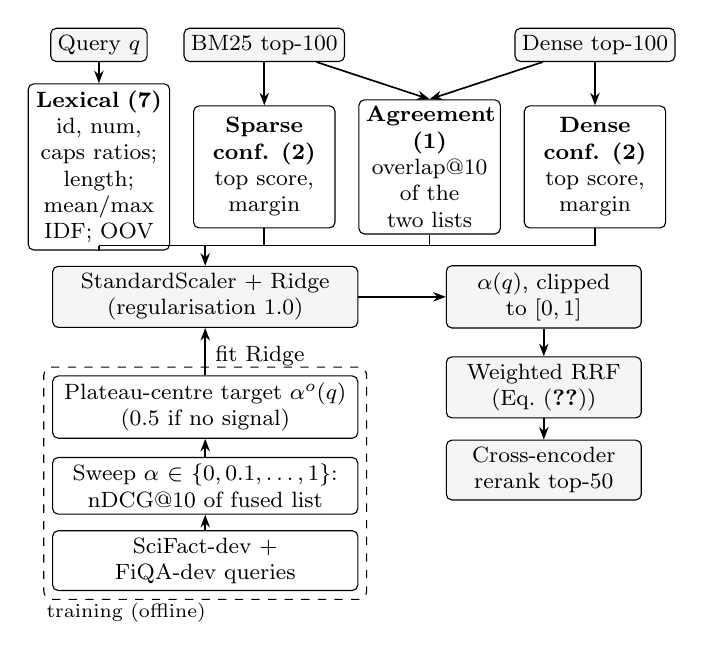
\begin{tikzpicture}[
  font=\footnotesize,
  box/.style={draw, rounded corners=2pt, align=center, inner sep=2.5pt, fill=gray!8},
  feat/.style={box, fill=white, text width=1.62cm, minimum height=1.55cm},
  train/.style={box, fill=white, text width=3.7cm},
  arr/.style={-{Stealth[length=1.6mm]}, semithick}]
  % inputs
  \node[box] (q)  at (0.95,0) {Query $q$};
  \node[box] (sp) at (3.05,0) {BM25 top-100};
  \node[box] (de) at (7.25,0) {Dense top-100};
  % feature groups from qaf.FEATURE_NAMES (agreement drawn between the two lists)
  \node[feat] (lex) at (0.95,-1.55) {\textbf{Lexical (7)}\\id, num, caps ratios; length; mean/max IDF; OOV};
  \node[feat] (sc)  at (3.05,-1.55) {\textbf{Sparse conf. (2)}\\top score, margin};
  \node[feat] (dc)  at (7.25,-1.55) {\textbf{Dense conf. (2)}\\top score, margin};
  \node[feat] (ag)  at (5.15,-1.55) {\textbf{Agreement (1)}\\overlap@10 of the two lists};
  \draw[arr] (q) -- (lex);
  \draw[arr] (sp) -- (sc);
  \draw[arr] (sp) -- (ag.north);
  \draw[arr] (de) -- (dc);
  \draw[arr] (de) -- (ag.north);
  % model
  \node[box, text width=3.7cm] (ridge) at (2.3,-3.2) {StandardScaler + Ridge\\(regularisation 1.0)};
  \node[box, text width=2.3cm] (clip)  at (6.6,-3.2) {$\alpha(q)$, clipped\\to $[0,1]$};
  % feature bus: all 12 features go into the scaler + ridge
  \foreach \n in {lex,sc,ag,dc} \draw[semithick] (\n.south) -- (\n.south |- 0,-2.55);
  \draw[semithick] (lex.south |- 0,-2.55) -- (dc.south |- 0,-2.55);
  \draw[arr] (ridge.north |- 0,-2.55) -- (ridge.north);
  \draw[arr] (ridge) -- (clip);
  \node[box, text width=2.3cm] (rrf) at (6.6,-4.35) {Weighted RRF\\(Eq.~\eqref{eq:rrf})};
  \node[box, text width=2.3cm] (rr)  at (6.6,-5.4)  {Cross-encoder\\rerank top-50};
  \draw[arr] (clip) -- (rrf);
  \draw[arr] (rrf) -- (rr);
  % training (offline)
  \node[train] (t3) at (2.3,-4.6) {Plateau-centre target $\alpha^{o}(q)$\\(0.5 if no signal)};
  \node[train] (t2) at (2.3,-5.6) {Sweep $\alpha\in\{0,0.1,\dots,1\}$:\\nDCG@10 of fused list};
  \node[train] (t1) at (2.3,-6.55) {SciFact-dev + FiQA-dev queries};
  \draw[arr] (t1) -- (t2);
  \draw[arr] (t2) -- (t3);
  \draw[arr] (t3) -- node[right, pos=0.4]{fit Ridge} (ridge);
  \node[draw, dashed, rounded corners=3pt, inner sep=3pt, fit=(t1)(t2)(t3)] (tr) {};
  \node[anchor=north west, inner sep=1pt] at (tr.south west) {\scriptsize training (offline)};
\end{tikzpicture}
\caption{QAF at query time (top and right) and its offline training (dashed
box). The four feature groups together hold the 12 features of
Table~\ref{tab:features}.}
\label{fig:qaf}
\end{figure}


\begin{table}[t]
\centering
\caption{QAF query features. The query is split into alphanumeric tokens
(compounds kept whole); ``ratio'' means the share of those tokens.}
\label{tab:features}
\footnotesize
\begin{tabular}{@{}>{\raggedright\arraybackslash}p{0.30\columnwidth}>{\raggedright\arraybackslash}p{0.64\columnwidth}@{}}
\toprule
Feature & Definition \\
\midrule
\texttt{id\_ratio} & identifier-like tokens: letters mixed with digits, an internal \texttt{\_-./}, or all capitals \\
\texttt{num\_ratio} & tokens made only of digits \\
\texttt{caps\_ratio} & all-capital tokens of length $\ge 2$ (acronyms) \\
\texttt{len\_tokens} & number of tokens \\
\texttt{mean\_idf}, \texttt{max\_idf} & BM25 IDF of the query terms in the target corpus \\
\texttt{oov\_ratio} & tokens absent from the dense encoder's tokenizer vocabulary (whole-word entries) \\
\texttt{sparse\_top}, \texttt{sparse\_margin} & top BM25 score and its gap to the second \\
\texttt{dense\_top}, \texttt{dense\_margin} & top cosine score and its gap to the second \\
\texttt{overlap\_at10} & share of the dense top-10 also in the sparse top-10 \\
\bottomrule
\end{tabular}
\end{table}

\textit{Training target.} For a labelled training query we sweep $\alpha$ over
$\{0,0.1,\dots,1\}$ and compute nDCG@10 of the fused list at each value. Since
Eq.~\eqref{eq:rrf} uses ranks only, nDCG is piecewise constant in $\alpha$ and
the optimum is usually a run of equally good grid points. Taking the first or
last maximiser would push targets toward the ends of the range for no real
reason, so the oracle $\alpha^{o}(q)$ is the centre of the longest contiguous
run of grid values that reach the best nDCG@10; between equally long runs we
keep the one nearer $0.5$. A query with nDCG@10 of zero at every $\alpha$
carries no signal and gets $0.5$.

\textit{Model and cost.} Standardised features feed a ridge regression
(regularisation $1.0$) whose output, clipped to $[0,1]$, is used as $\alpha$.
We fit one model per encoder on the pooled SciFact and FiQA dev queries; the
RFC and HotpotQA collections are never seen in training. We chose a linear
model so that its coefficients can be read and checked against intuition.
Every feature comes from the query, the two candidate lists, the BM25
document frequencies or, for \texttt{oov\_ratio}, the encoder's tokenizer
vocabulary, so QAF adds feature extraction and a 12-term dot product, with no
model call.

\subsection{Reranking, post-processing and generation}
The first 50 passages of the fused list are rescored by the BGE-reranker-base
cross-encoder, which reads query and passage (title and text, up to 512 tokens)
jointly as in monoBERT~\cite{nogueira2019passage}; the top five passages of the
new order form the context. The interactive pipeline can also drop near
duplicates (Jaccard similarity of word 5-gram sets $\ge 0.9$) and apply a
metadata filter before reranking; both are disabled in the reported
experiments. Optional query expansion, used only in the ablation, asks the
local LLM for at most 20 keywords or synonyms and appends them to the query.

Answers come from Qwen2.5-7B-Instruct~\cite{qwen2024qwen25} served by Ollama
at temperature 0 with a fixed seed. The prompt numbers the passages
\texttt{[1]}--\texttt{[5]} and asks for a short answer citing them in that
form, or the exact reply ``not in context'' when they do not support one.
Cited numbers are mapped back to passage ids, so we can check whether a cited
passage is relevant.

\section{Experimental Setup}
\label{sec:setup}

\subsection{Datasets}
\label{sec:data}
We use four test collections: SciFact (5{,}183 passages, 300 test queries),
a FiQA subset (20{,}000; 648), HotpotQA distractor paragraphs (4{,}955; 500)
and our RFC set (2{,}973 chunks; 101). Table~\ref{tab:dataset_stats} gives
dev-query counts, lengths and relevant passages per query; dev queries only
fit QAF and choose $\alpha^{*}$.
\inputtable{dataset_stats}

\textit{SciFact}~\cite{wadden2020scifact} and \textit{FiQA}~\cite{maia2018fiqa}
come from BEIR~\cite{thakur2021beir}. SciFact has no dev split, so we hold out
a seeded 20\% of its training queries. To keep encoding time manageable we
index 20{,}000 of FiQA's 57{,}638 posts: every post judged relevant for a dev
or test query (2{,}944) plus a seeded random sample of the rest. FiQA scores
are therefore not comparable with full-corpus BEIR numbers.
\textit{HotpotQA}~\cite{yang2018hotpotqa}: 500 seeded questions from the
distractor validation set; the corpus is the union of their paragraphs,
deduplicated by title, and the supporting paragraphs are relevant. It also
supplies gold answers for the generation experiments.

\textit{RFC corpus.} This collection targets questions about exact
identifiers; Fig.~\ref{fig:rfcdata} summarises how it was built. It holds 20 IETF
RFCs, from IP and TCP (RFC~791, 793) through DNS, HTTP/1.1, URI syntax, IPv6,
SMTP, WebSocket, OAuth~2.0, JWT, JSON and TLS~1.3 to QUIC and the 2022 HTTP
documents (RFC~9110, 9112, 9113). After removing page headers and footers, the
chunker of Section~\ref{sec:chunking} yields 2{,}973 chunks. Each question's
answer (at most eight words) is copied verbatim from its chunk; the filters
reject, among others, answers that occur more than once in their chunk or more
than three times in the parent RFC, and all three authors checked every
surviving draft against the RFC text. A typical question asks for the length
of the interface identifier in IPv6 unicast addresses (``64 bits''). A chunk
is relevant if its character span overlaps the answer span.

\begin{figure}[t]
\centering
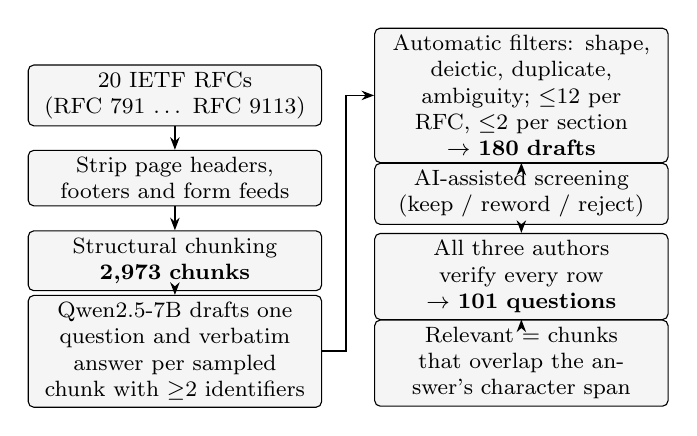
\begin{tikzpicture}[
  font=\footnotesize,
  box/.style={draw, rounded corners=2pt, align=center, inner sep=2.5pt, fill=gray!8, text width=3.55cm},
  arr/.style={-{Stealth[length=1.6mm]}, semithick}]
  \node[box] (a) at (1.95,0)    {20 IETF RFCs\\(RFC 791 \ldots\ RFC 9113)};
  \node[box] (b) at (1.95,-1.05) {Strip page headers, footers and form feeds};
  \node[box] (c) at (1.95,-2.1) {Structural chunking\\\textbf{2,973 chunks}};
  \node[box] (d) at (1.95,-3.25) {Qwen2.5-7B drafts one question and verbatim answer per sampled chunk with $\ge$2 identifiers};
  \node[box] (e) at (6.35,0)    {Automatic filters: shape, deictic, duplicate, ambiguity; $\le$12 per RFC, $\le$2 per section\\$\rightarrow$ \textbf{180 drafts}};
  \node[box] (f) at (6.35,-1.25) {AI-assisted screening\\(keep / reword / reject)};
  \node[box] (g) at (6.35,-2.3) {All three authors verify every row\\$\rightarrow$ \textbf{101 questions}};
  \node[box] (h) at (6.35,-3.4) {Relevant = chunks that overlap the answer's character span};
  \draw[arr] (a) -- (b);
  \draw[arr] (b) -- (c);
  \draw[arr] (c) -- (d);
  \draw[arr] (d.east) -- ++(0.3,0) |- (e.west);
  \draw[arr] (e) -- (f);
  \draw[arr] (f) -- (g);
  \draw[arr] (g) -- (h);
\end{tikzpicture}
\caption{Construction of the RFC test set. The filters run while questions
are generated; generation stops once 180 drafts have passed them.}
\label{fig:rfcdata}
\end{figure}

\subsection{Configurations}
For every collection and encoder we run \textbf{BM25} and \textbf{Dense}
alone; \textbf{Hybrid-fixed}, i.e.\ Eq.~\eqref{eq:rrf} with one weight
$\alpha^{*}$; \textbf{QAF}; both hybrids followed by reranking
(\textbf{+RR}); and an \textbf{Oracle} that uses each query's plateau-centre
oracle $\alpha$ (Section~\ref{sec:qaf}) computed on the test labels. Because the
centre of a plateau can fall between grid points, this is not a strict upper
bound; we use it as a reference for how much headroom per-query weighting has,
and report QAF's gap to it. $\alpha^{*}$ is the grid
value with the best mean nDCG@10 over the pooled SciFact and FiQA dev queries
(ties go to the value nearest 0.5) and is applied unchanged to all test sets
($\alpha^{*}=\AlphaStarBge$ for BGE, $\AlphaStarGemma$ for EmbeddingGemma~2).
We also sweep the fixed $\alpha$ over the grid on every test set.
The ablation, on SciFact and RFC with EmbeddingGemma~2, removes one component
at a time from the full system (structural chunks, QAF, reranking): QAF is
replaced by $\alpha^{*}$, reranking is dropped, and on RFC the structural
chunks are replaced by fixed 256-word windows, with relevance re-derived from
answer-span overlap. Query expansion is implemented but was not evaluated.
For the embedding-size study we truncate the stored EmbeddingGemma~2 vectors
to 512, 256 and 128 dimensions, renormalise them, rebuild the HNSW index with
the same settings, and retrain QAF and re-select $\alpha^{*}$ on the pooled
dev queries at each size. Answers are generated with EmbeddingGemma~2 for
BM25, Dense, Hybrid-fixed+RR and QAF+RR on \GenN{} sampled HotpotQA questions
and all 101 RFC questions.

\subsection{Metrics}
Retrieval is scored with Recall@$k$ ($k\in\{5,10,20\}$), MRR@10 and
\begin{equation}
  \mathrm{nDCG@}k=\frac{1}{\mathrm{IDCG@}k}\sum_{i=1}^{k}\frac{2^{\mathit{rel}_i}-1}{\log_2(i+1)},
  \label{eq:ndcg}
\end{equation}
where $\mathit{rel}_i$ is the graded relevance at rank $i$ and IDCG@$k$ is the
same sum for the ideal ordering~\cite{jarvelin2002ndcg}. A query with no
returned passages scores zero rather than being dropped. Answers are scored by
SQuAD-style~\cite{rajpurkar2016squad} exact match (EM) and token F1 after
lowercasing and removing punctuation and articles; the \texttt{[n]}
citation markers are stripped first. We also record whether a cited passage
is relevant (``Cite''). As a side analysis, RAGAS~\cite{es2024ragas}
faithfulness is scored for Dense and QAF+RR on the first \RagasN{} HotpotQA
questions (by id), with Qwen2.5-7B as judge. Every gain is reported as a mean per-query difference in nDCG@10 with a 95\%
paired-bootstrap confidence interval (10{,}000 resamples, seed 42) and tested
with a one-sided paired bootstrap and paired $t$-test at level $0.05$.

\subsection{Implementation and hardware}
Everything runs on one Apple M5 MacBook with 32\,GB of memory, with encoders
and reranker on PyTorch's MPS backend, the LLM in Ollama, and no paid API. The
code uses Python~3.12, sentence-transformers, FAISS, bm25s and scikit-learn.
Encoding dominates offline cost: EmbeddingGemma~2 encodes about
\GemmaDocsPerSec{} passages per second and BGE-small \BGEDocsPerSec{}, so
encoding the FiQA subset with the larger model takes about
\FiQAEncodeMinGemma{} minutes. All fusion variants are derived from cached
top-100 lists, which a test confirms match the end-to-end pipeline. All
sampling uses seed 42.

\section{Results}
\label{sec:results}
% Every number in this section comes from tables/*.tex, figures/*.pdf or a
% numbers.tex macro.

Tables~\ref{tab:main_results} and~\ref{tab:significance} give retrieval
scores and paired tests. ``Gain'' means the mean per-query difference in
nDCG@10; headline numbers use EmbeddingGemma~2, the encoder with the better
pooled-dev score for Hybrid-fixed. Our BM25 reaches
\BMndcgSciFact{} nDCG@10 on SciFact, close to the BM25 figure reported for
BEIR~\cite{thakur2021beir}, which we take as a check that indexing and
evaluation are sound.

\inputtable{main_results}
\inputtable{significance}

\subsection{Hybrid fusion against single retrievers}
Fixed-weight fusion is significantly better than the stronger single
retriever on FiQA with both encoders, and on SciFact and HotpotQA with
BGE-small (second block of Table~\ref{tab:significance}). FiQA shows that the
two sides need not be equally strong: BM25 is far behind dense there, yet
fusion still helps. With EmbeddingGemma~2, whose dense run is much stronger
(\BestNDCGSciFact{} on SciFact), fusion significantly lowers SciFact and is
level on HotpotQA (same block). On RFC, BM25 is the best single retriever,
well ahead of either dense encoder; Hybrid-fixed without reranking differs
from it by \HybridGainOverBMRFC{} and from dense by \HybridGainOverDenseRFC. Fig.~\ref{fig:alpha_sweep} shows why: SciFact and
HotpotQA improve toward the dense end, FiQA peaks in the interior, and RFC
peaks near the sparse end, so $\alpha^{*}=\AlphaStarGemma$, chosen on the SciFact
and FiQA dev queries, sits on the wrong side of the curve for RFC. At low
dense weights the RFC curve rises above BM25 alone, so the problem there is
the transferred weight, not fusion itself.

\inputfigure{alpha_sweep}{nDCG@10 of fixed-weight fusion as a function of the
dense weight $\alpha$ on each test collection (EmbeddingGemma~2, no
reranking).}

\subsection{Does query-adaptive fusion help?}
Not reliably. With EmbeddingGemma~2 and reranking, QAF+RR minus
Hybrid-fixed+RR is \QAFgainSciFact{} on SciFact (95\% CI
\QAFgainCISciFact), \QAFgainFiQA{} on FiQA (\QAFgainCIFiQA), \QAFgainHotpot{}
on HotpotQA (\QAFgainCIHotpot) and \QAFgainRFC{} on RFC (\QAFgainCIRFC,
$p=\QAFpRFC$). Only on RFC is the difference sizeable in QAF's favour, and even there the
interval includes zero. With BGE-small, QAF+RR wins narrowly on SciFact
(first block of Table~\ref{tab:significance}) and is ahead on RFC. The
per-query spread is wide on every
collection (standard deviation of nDCG@10 for QAF+RR: \NDCGsdSciFact{} on
SciFact, \NDCGsdRFC{} on RFC), so mean differences of this size are hard to
separate from noise with our query counts.

There is room for a better weight. The plateau-centre oracle, which picks
each query's weight from its own test labels, beats $\alpha^{*}$ by
\OracleHeadroomSciFact{} on SciFact and \OracleHeadroomRFC{} on RFC. It is
a headroom reference, not an upper bound, and QAF recovers little of it.

\subsection{What QAF learned}
The ridge model explains little of the variance in the oracle targets:
training $R^2$ is \QAFtrainRsq{} on \QAFnDev{} pooled dev queries with
EmbeddingGemma~2. Among the standardised coefficients, the largest
belongs to \QAFtopFeature: a confident dense retriever pushes the weight
toward the dense side. Several features push it the other way, among them the
BM25 margin, the overlap between the two lists and, less intuitively, the
dense margin. The identifier share, which motivated the method,
has a coefficient close to zero. As a result, predictions stay close to the
intercept: on the test queries the predicted weight has mean \QAFpredMean{}
and standard deviation \QAFpredSd{}, and identifier-heavy queries get almost
the same distribution as natural-language ones. In practice QAF behaves like a
constant that has been shrunk from $\alpha^{*}=\AlphaStarGemma$ toward the
middle of the range. That shift is probably what helps on RFC, whose sweep
favours the sparse side, more than any recognition of identifier queries.
The targets explain part of the difficulty: \QAFinsensitivePct\% of training queries
have the same nDCG@10 at every grid weight and therefore carry the neutral
target 0.5.

% Coefficient table (tables/qaf_coefficients.tex) omitted for space.

\subsection{Reranking and latency}
The cross-encoder is not a uniform win. Over QAF it adds large, significant
gains on HotpotQA and RFC with both encoders (third block of
Table~\ref{tab:significance}), but it hurts strong first stages:
\RerankGainSciFact{} on SciFact with EmbeddingGemma~2, and a significant loss
on FiQA with BGE-small. A general-purpose reranker over the top 50 can undo a
good dense ranking when its notion of relevance differs from the collection's
labels. EmbeddingGemma~2's dense SciFact score may also be helped by overlap
between its training data and this public benchmark, which we cannot check.

Reranking dominates cost: with EmbeddingGemma~2 it takes \RerankLatencyMs{}~ms
of the \TotalLatencyMs{}~ms mean per-query latency of QAF+RR, while the QAF
decision takes \QAFlatencyMs{}~ms.

\subsection{Statistical caveats}
Table~\ref{tab:significance} reports 28 one-sided tests without correction
for multiple comparisons. Under a Bonferroni threshold of $0.05/28$, only the
results with $p<0.0001$ would survive: Hybrid-fixed over the best single
retriever on FiQA with EmbeddingGemma~2, reranking on HotpotQA with both
encoders and on RFC with BGE-small, and EmbeddingGemma~2 over BGE-small on
HotpotQA. None of the QAF comparisons survive. FiQA scores come from a
20{,}000-passage subset that keeps every dev and test positive, so only
relative comparisons on FiQA are meaningful.

\subsection{Ablation}
Table~\ref{tab:ablation} removes one component at a time from the full
EmbeddingGemma~2 system. Dropping the reranker raises SciFact, in line with
the reranking results above, but costs RFC most of its gain. Replacing QAF by
$\alpha^{*}$ changes little: SciFact moves slightly up and RFC slightly down.
On RFC, fixed 256-word windows score clearly below structural chunks. This
comparison changes two things at once, chunk boundaries and the size of the
retrieval unit, and its relevance labels were re-derived from answer spans,
so we read it as evidence for structure-aware chunking on RFC rather than as
a clean measurement of it. Query expansion was not evaluated.

\inputtable{ablation}

\subsection{Embedding size}
Truncating EmbeddingGemma~2 hurts dense retrieval gradually. From 768 to 256
dimensions dense nDCG@10 drops by \MatryoshkaDropTwoFiftySix{} on average over
SciFact and RFC, with RFC losing more, and the loss grows at 128
(Table~\ref{tab:matryoshka}). After fusion and reranking the curve is almost
flat, so on these two collections a 256-dimensional index costs nothing
measurable in the full pipeline.
The index file shrinks less than the dimension does, because the HNSW graph,
which does not depend on the dimension, is part of it. Dense query latency
stays in the tens of milliseconds at every size (Table~\ref{tab:matryoshka})
and is dominated by query encoding.

\inputtable{matryoshka}

\subsection{Answer quality}
Answer quality does not follow retrieval quality on HotpotQA
(Table~\ref{tab:generation}). There, Dense gives the best answers and is
significantly better in F1 than Hybrid-fixed+RR, although the reranked hybrids
retrieve better. On RFC the two hybrid configurations give the best EM, F1 and
citation accuracy, ahead of Dense and BM25. QAF+RR is not significantly
better than Hybrid-fixed+RR on either collection. In the RAGAS side analysis
on HotpotQA, Dense answers are judged slightly more faithful than QAF+RR
answers (\FaithDense{} against \FaithQAF). The judge is the same 7B model that
wrote the answers, so this comparison may suffer from self-preference and we
give it little weight. A sheet of sampled answers for manual faithfulness labelling is provided
with the code; the team has not yet completed it.

\inputtable{generation}

\section{Discussion}
\label{sec:discussion}

\subsection{Why per-query weighting is hard to learn}
We expected identifier-heavy queries to want a low dense weight and cheap
features to detect them. The first half holds at the collection level, but the
identifier share carries almost no signal. Three factors likely contribute:
\QAFinsensitivePct\% of training targets are uninformative because nDCG@10 does
not change with the weight; plateau centres on a coarse grid of a rank-based
fusion are noisy targets; and the model never saw text like RFC. In-domain
labels or post-retrieval evidence, as in DAT~\cite{hsu2025dat}, may close
more of the headroom; pre-retrieval statistics alone did not.

\subsection{Cost and deployment guidance}
Four practical points follow. Sweep $\alpha$ on a small labelled sample of
the target collection before fixing it, since a weight chosen on other domains
landed on the wrong side of the curve for RFC. Keep BM25 for identifier-heavy
text even with a strong dense encoder. Measure the reranker before adopting
it: on our laptop it multiplies latency many times over and lowered nDCG@10
where the first stage was already strong. QAF costs well under a millisecond,
but on our evidence it does not replace tuning. Finally, a 256-dimensional
EmbeddingGemma~2 index is a safe saving inside a reranked hybrid pipeline,
but not for dense retrieval on its own.

\subsection{Limitations}
All experiments run on subsets (FiQA 20{,}000 passages, HotpotQA 500 questions with their own
paragraphs as the corpus, RFC 101 questions), so absolute scores are not
comparable with full-benchmark numbers (Section~\ref{sec:results}). The RFC questions were drafted by Qwen2.5-7B, the same model that
generates answers, and every row was verified by all three authors, but the
set favours questions that a 7B model finds easy to write, namely
short identifier lookups without multi-hop items. RFC~2616, 7230 and
9110/9112 are successive HTTP/1.1 specifications with overlapping text, so a
near-duplicate passage from a superseded RFC counts as a miss, even though
questions ambiguous across RFCs were removed.

QAF was fitted on scientific and financial dev queries only, and we compare
it with a fixed weight and the oracle but not with an LLM-based scheme such as
DAT, so we cannot say how much accuracy the LLM-free design gives up. Query
expansion was implemented but not evaluated. The RAGAS judge is the same 7B
model that wrote the answers and covers only two configurations on
HotpotQA, and the manual faithfulness check is still pending, so we make no
claim about faithfulness beyond that side analysis. The 28 significance tests
are uncorrected, and RFC has only 101 questions. Latencies come from one
laptop and will differ elsewhere in absolute terms. We also cannot rule out
that EmbeddingGemma~2 saw SciFact or HotpotQA text during training, which would
flatter its dense scores there.

\section{Conclusion}
\label{sec:conclusion}
We built a hybrid RAG pipeline that runs entirely on a laptop and asked
whether the dense/sparse balance should be set per query. Fixed-weight fusion helps
unless the dense model is much stronger or the weight was tuned on other
collections; on identifier-heavy RFC text, BM25 beat the dev-tuned hybrid. Our LLM-free QAF model is cheap and readable but does not
reliably beat a fixed weight, behaving mostly like a shrunk constant, although
the oracle headroom is real. Answers from a local 7B generator do not simply
track retrieval quality: hybrids gave the best answers on RFC, dense retrieval
on HotpotQA. Next we plan to compare against LLM-based weighting such as DAT and to
add post-retrieval features to the weight predictor.


\section*{Acknowledgment}
We thank our supervisor, Dr Rajat Takkar, Department of Computer Science and
Engineering, Chitkara University, for his guidance throughout this project.

\bibliographystyle{IEEEtran}
\bibliography{refs}

\end{document}
